\documentclass[12pt]{article}
\usepackage[utf8]{inputenc}

\usepackage{lmodern}

\usepackage{enumitem}
\usepackage[margin=2cm]{geometry}

\usepackage{amsmath, amsfonts, amssymb}
\usepackage{graphicx}
%\usepackage{subfigure}
\usepackage{tikz}
\usepackage{pgfplots}
\usepackage{multicol}

\usepackage{comment}
\usepackage{url}
\usepackage{calc}
\usepackage{subcaption}
\usepackage[indent=0pt]{parskip}
\usepackage{animate}

\usepackage{array}
\usepackage{blkarray,booktabs, bigstrut}
\usepackage{bigints}

\pgfplotsset{compat=1.16}

% MATH commands
\newcommand{\ga}{\left\langle}
\newcommand{\da}{\right\rangle}
\newcommand{\oa}{\left\lbrace}
\newcommand{\fa}{\right\rbrace}
\newcommand{\oc}{\left[}
\newcommand{\fc}{\right]}
\newcommand{\op}{\left(}
\newcommand{\fp}{\right)}

\newcommand{\bi}{\mathbf{i}}
\newcommand{\bj}{\mathbf{j}}
\newcommand{\bk}{\mathbf{k}}
\newcommand{\bF}{\mathbf{F}}

\newcommand{\mR}{\mathbb{R}}

\newcommand{\ra}{\rightarrow}
\newcommand{\Ra}{\Rightarrow}

\newcommand{\sech}{\mathrm{sech}\,}
\newcommand{\csch}{\mathrm{csch}\,}
\newcommand{\curl}{\mathrm{curl}\,}
\newcommand{\dive}{\mathrm{div}\,}

\newcommand{\ve}{\varepsilon}
\newcommand{\spc}{\vspace*{0.5cm}}

\DeclareMathOperator{\Ran}{Ran}
\DeclareMathOperator{\Dom}{Dom}

\newcommand{\exo}[1]{\noindent\textcolor{red}{\fbox{\textbf{Problem {#1}}}\hrulefill}\\}
\newcommand{\qu}[4]{\noindent\textcolor{#4}{\fbox{\textbf{Section {#1} | Problem {#2}}} \hrulefill{{\fbox{\textbf{{#3} Points}}}}\\}}

\newcommand{\semester}{Spring 2023}

\newcommand{\CVup}{%
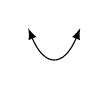
\begin{tikzpicture}
\draw[black, <->, >=latex] (-0.33, 0.5) .. controls (-0.125, 0) and (0.125, 0) .. (0.33, 0.5);
\end{tikzpicture}}

\newcommand{\CVupInc}{%
\begin{tikzpicture}
\draw[black, ->, >=latex] (0,0) .. controls (0.2, 0) and (0.4, 0.2) .. (0.5, 0.5);
\end{tikzpicture}}

\newcommand{\CVupDec}{%
\begin{tikzpicture}[rotate=270]
\draw[black, ->, >=latex] (0,0) .. controls (0.2, 0) and (0.4, 0.2) .. (0.5, 0.5);
\end{tikzpicture}}

\newcommand{\CVdown}{%
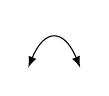
\begin{tikzpicture}
\draw[black, <->, >=latex] (-0.33, -0.5) .. controls (-0.125, 0) and (0.125, 0) .. (0.33, -0.5);
\end{tikzpicture}}

\newcommand{\CVdownInc}{%
\begin{tikzpicture}
\draw[black, ->, >=latex] (-0.5, -0.5) .. controls (-0.5, -0.3) and (-0.5, -0.1) .. (0,0);
\end{tikzpicture}}

\newcommand{\CVdownDec}{%
\begin{tikzpicture}[rotate=-90]
\draw[black, ->, >=latex] (-0.5, -0.5) .. controls (-0.5, -0.3) and (-0.5, -0.1) .. (0,0);
\end{tikzpicture}}

\begin{document}
	\noindent \hrulefill \\
	MATH-241 \hfill Pierre-Olivier Paris{\'e}\\
	Solutions Section 5-2 \hfill \semester \\\vspace*{-1cm}
	
	\noindent\hrulefill
	
	\spc
	
	\exo{6}
	\\
	The curve is a parabola, $x = y^2/2$. The $y$ values are bounded by $y = 0$ (because $x = 0$ implies that $y = 0$) and $y = 4$. Therefore, the region is given by $0 \leq x \leq y^2/2$ and $0 \leq y \leq 4$.
	\begin{center}
	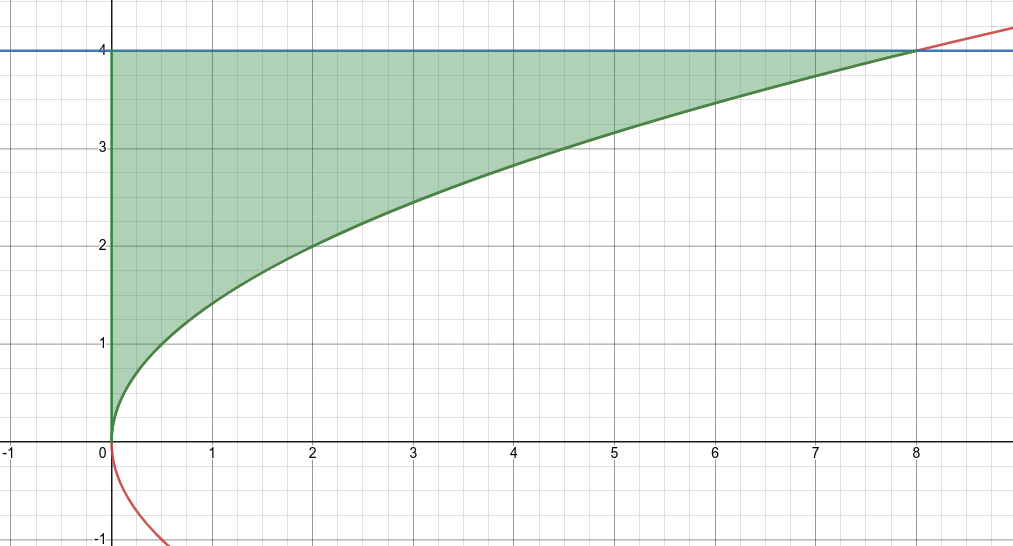
\includegraphics[scale=0.3]{fig3.png}
	\end{center}
	
	The rotation is about the $y$-axis. We therefore draw a small horizontal rectangle with height $dy$ and width $x$.
	
	\begin{center}
	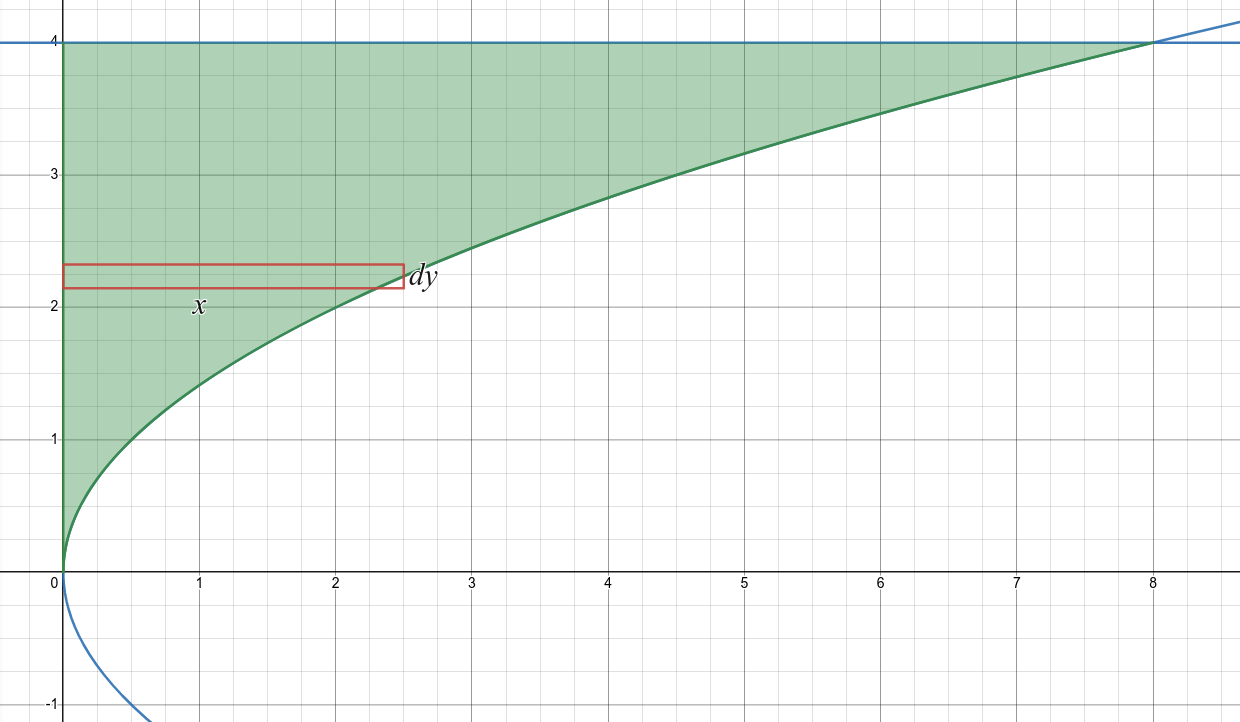
\includegraphics[scale=0.3]{fig4.png}
	\end{center}
	
	After rotation, the radius of the disk created is $x$ and the height is $dy$. Therefore, the volume is
		\begin{align*}
		\int_0^4 \pi (\text{radius})^2 dy = \int_0^4 \pi x^2 \, dy .
		\end{align*}
	But now, $x = y^2/2$, and therefore
		\begin{align*}
		\int_0^4 \pi x^2 \, dy = \int_0^4 \pi \frac{y^4}{4} \, dy =  \pi \left. \big( \frac{y^5}{20} \big) \right|_0^4 = \frac{256\pi}{5} .
		\end{align*}
		
	\newpage
	
	\exo{8}
	\\
	Here is the sketch of the region to rotate about the $x$-axis and a gif of the rotation\footnote{The gif will work if you open the pdf with Adobe Acrobat Reader.}:
		\begin{figure}[h]
		\begin{subfigure}[b]{0.45\textwidth}
		\centering
		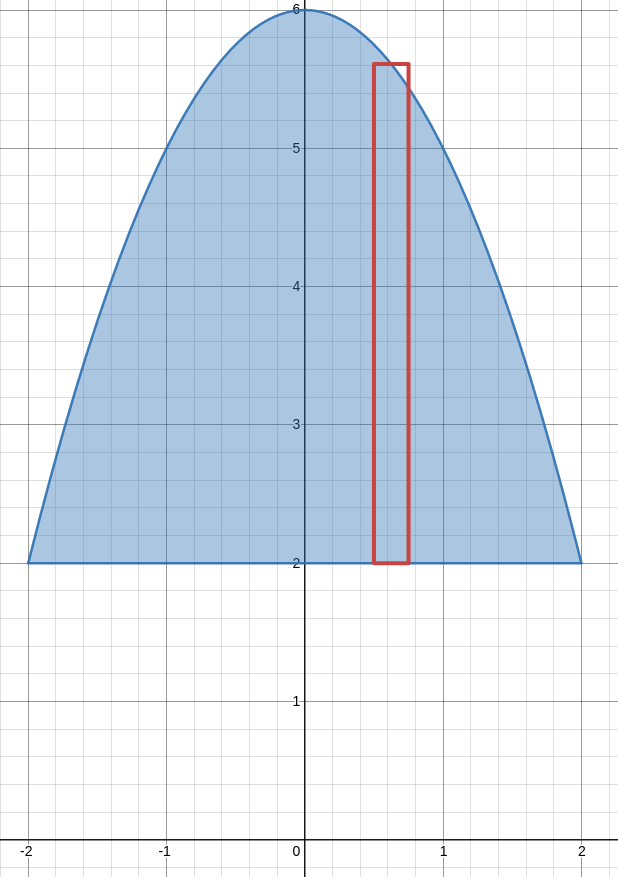
\includegraphics[scale=0.3]{exo8_52}
		\caption{Region to rotate}
		\end{subfigure}
		\begin{subfigure}[b]{0.45\textwidth}
		\animategraphics[scale=0.75]{20}{python/Revolution}{0}{200}
		\caption{Rotation of the region}
		\end{subfigure}
		\end{figure}
		
	We will use the washer method. The inner radius is $r_{in} = y = 2$ and the outer radius is $r_{out} = y = 6 - x^2$. The values of $x$ start at $x = -2$ and ends at $x = 2$. So, by the washer method, we obtain
		\begin{align*}
		V (S) = \int_{-2}^2 \pi r_{out}^2 - \pi r_{in}^2 \, dx = \pi \int_{-2}^2 ((6 - x^2)^2 - 2^2 ) \, dx = 384/5 .
		\end{align*}
	
\end{document}